	\chapter{Natural Language Processing}
	\section{Frequently Asked Questions}

	\resetquestioncounter{}
	\begin{qanda}
		\begin{question}
 What are the fields of NLP?
 		\end{question}
		\begin{answer}
			\begin{bulletedlist}
				\item Speech Recognition - The translation of spoken language into text.
				\item Natural Language Understanding - The computer's ability to understand what we say.
				\item Natural Language Generation - The generation of natural language by a computer.
			\end{bulletedlist}
		\end{answer}
	\end{qanda}

	\begin{qanda}
		\begin{question}
What are the Major Challenges of Natural Language Processing (NLP)?
		\end{question}
		\begin{answer}
Natural Language Processing (NLP) Challenges:\\
{\small \url{https://monkeylearn.com/blog/natural-language-processing-challenges/}}
		\end{answer}
	\end{qanda}

	\begin{qanda}
		\begin{question}
What are all the different text pre-processing steps to perform different NLP Tasks?
		\end{question}
		\begin{answer}
A comprehensive introduction to text preprocessing, covering the different techniques including stemming, lemmatization, noise removal, and normalization, with examples and explanations about when you should use each of them:
\href{https://kavita-ganesan.com/text-preprocessing-tutorial/#.YtCThXbMImL}{Text Preprocessing for Machine Learning and NLP}
		\end{answer}
	\end{qanda}

	\begin{qanda}
		\begin{question}
How to remove numbers from a string in a Pandas DataFrame column?
		\end{question}
		\begin{answer}
You can use the below code and define a suitable function for it, iterate that over the DataFrame:

text = re.sub(r'\d+', '', text)
		\end{answer}
	\end{qanda}

	\begin{qanda}
		\begin{question}
I am able to import nltk library but get errors while performing operations based on it LookupError: Please use the NLTK Downloader to obtain the resource.
		\end{question}
		\begin{answer}
Run the below code and its dependency before performing the operations based on it.

			\begin{code}[\codenumbering]{}
				\codeitemnonumber import nltk \# Import Natural Language Tool-Kit.
				\codeitemnonumber nltk.download('stopwords') \# Download Stopwords.
				\codeitemnonumber nltk.download('punkt')
				\codeitemnonumber nltk.download('wordnet')
			\end{code}
		\end{answer}
	\end{qanda}

	\section{Introduction}
	\begin{bulletedlist}
		\item Natural Language Processing is a subfield of artificial intelligence concerned with methods of communication between computers and natural languages such as English, Hindi, etc.
		\item It is an intersection of fields of Computer Science, linguistics, and AI
		\item Objective of Natural Language processing is to perform useful tasks involving human languages like:
		\begin{bulletedlist}
			\item Sentiment Analysis
			\item Machine Translation
			\item Part of Speech Tags
			\item Human-Machine communication (chat-bots)
		\end{bulletedlist}
		\item Language is involved in most of the activities that involve interaction between humans, e.g. reading, writing, speaking, listening.
		\item Voice can be used as an interface for interactions between humans and machines e.g. Cortana, Google Assistant, Siri, Amazon Alexa.
		\item There is massive amount of data available in text format which can used to derive insights from using NLP, e.g. blogs, research articles, consumer reviews, literature, discussion forums.
	\end{bulletedlist}

	\subsection{Different Tasks in NLP}
	\begin{bulletedlist}
		\item Text Classification
		\begin{bulletedlist}
			\item Sentiment Analysis: Determining the general context of a review, whether it is positive or negative or neutral.
			\item Consumer Complaints Classification:
			\begin{bulletedlist}
				\item Categorizing complaints on consumer
				\item forums to respective departments.
			\end{bulletedlist}
		\end{bulletedlist}
		\item Machine Translation
		\begin{bulletedlist}
			\item Improving human-human interaction by translating sentences from one language to another.
		\end{bulletedlist}
		\item Part of Speech Tagging
		\begin{bulletedlist}
			\item In corpus linguistics, part-of-speech tagging (POS tagging or PoS tagging or POST), also called grammatical tagging or word-category disambiguation, is the process of marking up a word in a text (corpus) as corresponding to a particular part of speech, based on both its definition and its context.
			\item A simplified form of this is the identification of words as nouns, verbs, adjectives, adverbs, etc.
			\item \href{Tag-set}{https://www.ling.upenn.edu/courses/Fall\_2003/ling001/penn\_treebank\_pos.html}
		\end{bulletedlist}
		\item Word Segmentation
		\begin{bulletedlist}
			\item In some languages, there is no space between words, or a word may contain smaller syllables. In such languages, word segmentation is the first step of NLP systems.
		\end{bulletedlist}
		\item Semantic Analysis
		\begin{bulletedlist}
			\item Semantic analysis of a corpus (a large and structured set of texts) is the task of building structures that approximate concepts from a large set of documents.
			\item Application of Semantic Analysis
			\begin{bulletedlist}
				\item
				\begin{bulletedlist}
					\item Categorizing complaints on consumer
					\item forums to respective departments.
				\end{bulletedlist}
			\end{bulletedlist}
		\end{bulletedlist}
	\end{bulletedlist}

	\subsection{Difficulties of NLP}
	\begin{bulletedlist}
		\item Languages are changing everyday, new words, new rules, etc.
		\item The number of tokens is not fixed. A natural language can have hundreds of thousands of different words, new words are created on the fly.
		\item Words can have different meanings depending on context, and they can acquire new meanings over time (apple(a fruit), Apple(the company)], they can even change their parts of speech(Google--> to google).
		\item Every language has its own uniqueness. Like in the case of English we have words, sentences, paragraphs and so on to limit our language. But in Thai, there is no concept of sentences.
	\end{bulletedlist}

	\subsection{Standard NLP Terms}
	\begin{bulletedlist}
		\item Corpus: A body of text samples
		\item Document: A text sample
		\item Vocabulary: A list of words used in the corpus
		\item Language model: How the words are supposed to be organized
	\end{bulletedlist}

	\section{Pre-processing Steps}
	\subsection{Why do we need pre-processing}
	\begin{bulletedlist}
		\item Textual data is unstructured and cannot be processed as it is.
		\item Text data also contains a lot of non- required items such as special characters, punctuations etc.
		\item We clean up the text corpus to make it processable by ML.
		\item This text clean-up process is called text pre-processing.
	\end{bulletedlist}

	\subsection{Text Analytics Framework}
	\begin{bulletedlist}
		\item NLTK: The Natural Language Toolkit is a complete platform that contains more than 50 corpora and lexical resources. It also provides the necessary tools, interfaces, and methods to process and analyze text data.
		\item Beautiful Soup : It can be used to scrape data from web and also for text cleaning with its inbuilt parsers.
		\item TextBlob: Provides several capabilities including text processing, phrase extraction, classification, POS tagging, text translation and sentiment analysis.
		\item Spacy : It is a production grade NLP library that offers similar functionality as that of NLTK and TextBlob
	\end{bulletedlist}

	\subsection{Types of Processing Steps}
	\begin{bulletedlist}
		\item Often, unstructured text contains a lot of noise, especially if you use techniques like web or screen scraping. HTML tags are typically one of these components which don't add much value towards understanding and analyzing text.
		\begin{bulletedlist}
			\item strip\_html\_tags('<html><h2>Some important text</h2></html>')
		\end{bulletedlist}
		\item Usually in any text corpus, you might be dealing with accented characters/letters, especially if you only want to analyze the English language.  Hence, we need to make sure that these characters are converted and standardized into ASCII characters.
A simple example - converting \'{e} to e.
		\begin{bulletedlist}
			\item remove\_accented\_chars('S\'{o}m\^{e} \'{A}ccent\^{e}d t\'{e}xt')
		\end{bulletedlist}
	\end{bulletedlist}

	\subsection{Removal of Special Characters}
	\begin{bulletedlist}
		\item Special characters and symbols are usually non-alphanumeric characters or even occasionally numeric characters (depending on the problem), which add to the extra noise in unstructured text.  Usually, simple regular expressions (regex) can be used to remove them.
		\begin{bulletedlist}
			\item remove\_special\_characters(``Well this was fun! What do you think? 123\#@!'', remove\_digits=True)
		\end{bulletedlist}
	\end{bulletedlist}

	\subsection{Tokenization}
	\begin{bulletedlist}
		\item Tokenization is the task of taking a text or set of text and breaking it up into its individual tokens.
		\item Tokens are usually individual words (at least in languages like English).
		\item Tokenization can be achieved using different methods. Most common method is Whitespace tokenizer and Regexp Tokenizer.
	\end{bulletedlist}

	\subsection{Stop Words Removal}
	\begin{bulletedlist}
		\item Stopwords are common words that carry less important meaning than keyword
		\item When using some bag of words based methods, i.e, countVectorizer or tf-idf that works on counts and frequency of the words, removing stop words is great as it lowers the dimensionality.
		\begin{bulletedlist}
			\item remove\_stopwords (``The, and, if are stop words, computer is not'')
			\item Removing stop words minimizes computation.
		\end{bulletedlist}
		\item Not always a good idea.
		\begin{bulletedlist}
			\item When working on problems where contextual information is important like machine translation, removing stop words is not
recommended.
		\end{bulletedlist}
	\end{bulletedlist}

	\begin{figure}[h]
		\centering
		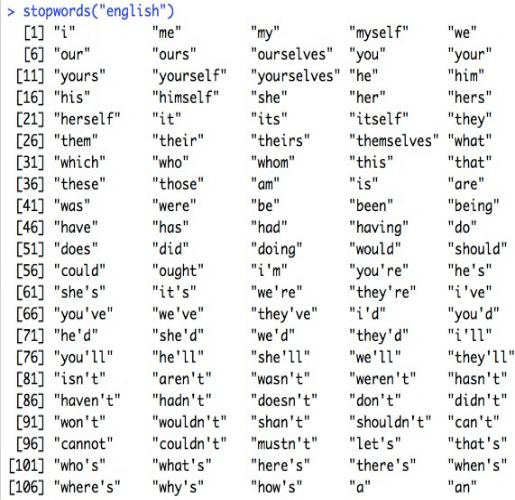
\includegraphics[height=2.5in]{stopwords}
		\caption[Stop words]{Stop words.}
		\label{fig:stopwords}
	\end{figure}


	\subsection{Stemming}
	\begin{bulletedlist}
		\item The idea of reducing different forms of a word to a core root.
		\item Words that are derived from one another can be mapped to a central word or symbol, especially if they have the same
core meaning.
		\item Used for dimensionality reduction.
		\item Word stem may not be present in dictionary.
		\item ``cook,'' ``cooking,'' and ``cooked'' all are reduced to same stem of ``cook.''
	\end{bulletedlist}

	\begin{figure}[h]
		\centering
		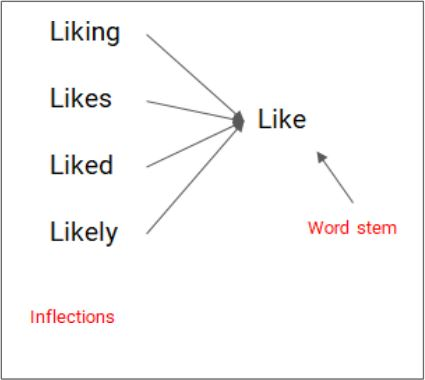
\includegraphics[height=1.5in]{wordstemming}
		\caption[Word stemming]{Word stemming.}
		\label{fig:wordstemming}
	\end{figure}


